\documentclass[11pt]{article}
\usepackage{amsmath,amssymb,amsthm,mathtools}
\usepackage[a4paper,margin=1in]{geometry}
\usepackage{bm}
\usepackage{xcolor}
\usepackage{hyperref}
\newtheorem{theorem}{Theorem}
\newtheorem{remark}[theorem]{Remark}
\title{DG formulation and Newton linearization
for a 1D embedded Blood Flow system with Lax--Friedrichs flux}
\author{}
\date{}

\newcommand{\R}{\mathbb{R}}
\newcommand{\avg}[1]{\left\{\!\!\left\{#1\right\}\!\!\right\}}
\newcommand{\jump}[1]{\left[\!\left[#1\right]\!\right]}
\newcommand{\dt}{\Delta t}
\newcommand{\Vh}{V_h}
\newcommand{\Th}{\mathcal{T}_h}
\newcommand{\Fh}{\mathcal{F}_h}
\newcommand{\Kh}{K}
\newcommand{\norm}[1]{\left\lVert #1\right\rVert}

\begin{document}
\maketitle

\section{Model problem and geometry}

We consider the one-dimensional blood flow equations embedded along a
centerline $\Gamma\subset\R^{\text{spacedim}}$, parameterized by a unit tangent
vector $\bm b(\bm x)$:
\begin{align}
  \partial_t A + \bm b\!\cdot\!\nabla (A U) &= 0,
  && \text{(Area equation)}, \label{eq:area-eq}\\[2mm]
  \partial_t U + \bm b\!\cdot\!\nabla\!\left(\frac{U^2}{2}\right)
  + \frac{1}{\rho}\bm b\!\cdot\!\nabla P(A)
  + c\,U &= 0,
  && \text{(Momentum equation).} \label{eq:momentum-eq}
\end{align}
Here $A$ and $U$ denote the cross-sectional area and mean velocity,
respectively.
The direction vector of each 1D element is
\[
  \bm b = \frac{\bm x_1 - \bm x_0}{\lVert \bm x_1 - \bm x_0\rVert},
  \qquad
  \beta = \bm b\!\cdot\!\bm n
\]
is its projection on the outward normal $\bm n$.
The pressure $P(A)$ is governed by a constitutive \emph{tube law},
for example
\[
  P(A) = P_0 + \mu \!\left[\!\left(\frac{A}{A_0}\right)^m - 1\!\right],
  \qquad
  \frac{dP}{dA} = \mu \,m\,\frac{A^{m-1}}{A_0^m},
\]
and the wave speed is
\[
  c = \sqrt{\frac{A}{\rho}\frac{dP}{dA}}.
\]

The compact vector form of the system is
\begin{equation}
  \partial_t \mathbf{W} + \bm b\!\cdot\!\nabla \mathbf{F}(\mathbf{W})
  = S(\mathbf{W}),
  \qquad
  \mathbf{W} =
  \begin{pmatrix} A \\[1mm] U \end{pmatrix},
  \quad
  S(\mathbf{W}) = -
  \begin{pmatrix} 0 \\[1mm] cU \end{pmatrix},
  \label{eq:model-vector}
\end{equation}
with the physical flux
\[
  \mathbf{F}(\mathbf{W}) =
  \begin{pmatrix}
    A U \\[2mm]
    \dfrac{U^2}{2} + \dfrac{1}{\rho} P(A)
  \end{pmatrix}.
\]


\section{Discontinuous Galerkin weak formulation}


Let $\Th$ denote a partition of $\Gamma$ into 1D elements $K$, and for
polynomial degree $k\ge0$ define the discontinuous finite element space
\[
  \Vh = \{v\in L^2(\Gamma): v|_K \in \mathbb P_k(K),\ \forall K\in\Th\}.
\]
For an interior face $F\in\Fh^\circ$ with unit normal $\bm n$,
the jump and average operators are
\[
  \jump{v}=v^- - v^+,
  \qquad
  \avg{v}=\tfrac12(v^-+v^+),
\]
and on boundary faces $F\subset\partial\Gamma$ we set
$\avg{v}=v$ and $\jump{v}=v$

DG weak form for \eqref{eq:model-vector} is 
\begin{equation}{\label{semi-discrete-weak-form}}
     \left( \partial_t \mathbf{W}_h , \phi \right)
  - (\mathbf{F}(\mathbf{W}), \bm b\!\cdot\!\nabla \phi) + \langle \widehat{\mathbf{F}}(\mathbf{W}), \bm b.n \, \phi \rangle
  - (S(\mathbf{W}_h), \phi) = 0,
\end{equation}
where $\widehat{\mathbf{F}}$ is numerical flux defined later.

\section{Newton iteration in time}

At each time step $t_{n+1}$, we must solve the nonlinear fully discrete DG system
\eqref{semi-discrete-weak-form}.
Using the backward Euler discretization, the discrete residual is defined as
\begin{equation}\label{def:residual-vector}
  \left(\mathcal{R}^{n+1}(\mathbf{W}_h^{n+1}), \phi\right)
  :=
  \left(\frac{\mathbf{W}_h^{n+1} - \mathbf{W}_h^n}{\dt}, \phi \right)
  - (\mathbf{F}(\mathbf{W}_h^{n+1}), \bm b\!\cdot\!\nabla \phi) + \langle \widehat{\mathbf{F}}(\mathbf{W}_h^{n+1}), \bm b.n \, \phi \rangle
  - (S(\mathbf{W}_h^{n+1}), \phi),
\end{equation}
and we seek $\mathbf{W}_h^{n+1}$ such that
$\mathcal{R}^{n+1}(\mathbf{W}_h^{n+1}) = 0$ in the weak DG sense.

\subsection*{Linearization by Newton’s method}

Let $\mathbf{W}_h^{n+1,(k)}$ denote the current Newton iterate at time level $t_{n+1}$,
and define the Newton correction
\[
  \delta\mathbf{W}_h^{n+1,(k)} :=
  \mathbf{W}_h^{n+1,(k+1)} - \mathbf{W}_h^{n+1,(k)}.
\]
Then the first-order Taylor expansion of the residual at $t_{n+1}$ gives
\begin{equation}\label{residual_vector}
 \boxed{
  \left(\mathcal{R}^{n+1}\!\left(\mathbf{W}_h^{n+1,(k)} + \delta\mathbf{W}_h^{n+1,(k)}\right), \phi\right)
  \approx
  \left( \mathcal{R}^{n+1}\!\left(\mathbf{W}_h^{n+1,(k)}\right), \phi \right)
  +\left( \mathcal{J}^{(k)}\,\delta\mathbf{W}_h^{n+1,(k)}, \phi \right) .}
\end{equation}
The corresponding Newton correction equation reads
\begin{equation}\label{main-equation}
  \mathcal{J}^{(k)}\,\delta\mathbf{W}_h^{n+1,(k)}
  = -\mathcal{R}^{n+1}\!\left(\mathbf{W}_h^{n+1,(k)}\right),
\end{equation}
followed by the update
\[
  \boxed{
  \mathbf{W}_h^{n+1,(k+1)}
  = \mathbf{W}_h^{n+1,(k)} + \omega\,\delta\mathbf{W}_h^{n+1,(k)},
  \qquad 0 < \omega \le 1.}
\]

 Differentiating this residual with respect to $\mathbf{W}$ in the direction
$\delta\mathbf{W}_h^{n+1,(k)}$ yields the weak form of the Jacobian action:
\begin{equation}\label{jacobian_weak}
\boxed{
\begin{aligned}
  \bigl(\mathcal{J}^{(k)}\delta\mathbf{W}_h^{n+1,(k)}, \phi\bigr)
  &=
  \int_{\Omega}
    \frac{1}{\Delta t}\,
    \delta\mathbf{W}_h^{n+1,(k)}\cdot\phi
  \;dx
  - \int_{\Omega}
    \Big(
      \mathbf{H}^{(k)}\,\delta\mathbf{W}_h^{n+1,(k)}
    \Big)
    \cdot(\bm b\!\cdot\!\nabla\phi)
  \;dx \\[2mm]
  &\quad
  - \int_{\Omega}
    \Big(
      \frac{\partial S}{\partial\mathbf{W}}
      (\mathbf{W}_h^{n+1,(k)})\,
      \delta\mathbf{W}_h^{n+1,(k)}
    \Big)\cdot\phi
  \;dx
  + \int_{\partial\Omega}
    \Big(
      \frac{\partial\widehat{\mathbf{F}}}{\partial\mathbf{W}}
      (\mathbf{W}_h^{n+1,(k)})\,
      \delta\mathbf{W}_h^{n+1,(k)}
    \Big)\cdot\phi\,ds.
\end{aligned}}
\end{equation}
The flux Jacobian matrix evaluated at the current iterate is
\[
  \mathbf{H}^{(k)}
  = \frac{\partial\mathbf{F}}{\partial\mathbf{W}}(\mathbf{W}_h^{n+1,(k)})
  =
  \begin{pmatrix}
    U_h^{n+1,(k)} & A_h^{n+1,(k)} \\[1mm]
    \dfrac{\big(c_h^{n+1,(k)}\big)^{2}}{A_h^{n+1,(k)}} & U_h^{n+1,(k)}
  \end{pmatrix},
  \qquad
  c_h^{n+1,(k)}
  = \sqrt{\frac{A_h^{n+1,(k)}}{\rho}\frac{dP}{dA}\!\big(A_h^{n+1,(k)}\big)}.
\]

The numerical flux function $\widehat{\mathbf{F}}(\mathbf{W}^-,\mathbf{W}^+)$
appearing on interior and boundary faces is chosen as the
\emph{local Lax--Friedrichs (Rusanov) flux}, defined by
\begin{equation}\label{LF_flux}
  \boxed{
  \widehat{\mathbf{F}}(\mathbf{W}^-,\mathbf{W}^+;\bm n)
  = 
  \frac{1}{2}\Big(
      \mathbf{F}(\mathbf{W}^-)(b \cdot n)^{-}
    + \mathbf{F}(\mathbf{W}^+) (b \cdot n)^{+}
  \Big)
  \;-\;
  \frac{1}{2}\,\alpha^{(k)}\,
  (\mathbf{W}^+ - \mathbf{W}^-  ),
  }
\end{equation}
where $\mathbf{W}^-$ and $\mathbf{W}^+$ denote the interior and exterior traces
of the state vector across a face with unit normal $\bm n$. And $(b\cdot n)^{-} = b|_{K} \cdot \hat{n}_{k} = b|_{K} \cdot \hat{n}$, $(b\cdot n)^{+} =  b|_{K'} \cdot \hat{n}_{K'} = - b|_{K'} \cdot \hat{n}_{k}$ with $K$ and $K'$ are neighboring elements.
The parameter $\alpha^{(k)}$ is a local estimate of the maximum wave speed,
computed at the current Newton iterate as $|b \cdot n| =1$
\[
  \alpha^{(k)}
  =
  \max\!\Big(
      \big|\lambda_1^{(k)}(\mathbf{W}^-)\big|,
      \big|\lambda_2^{(k)}(\mathbf{W}^-)\big|,
      \big|\lambda_1^{(k)}(\mathbf{W}^+)\big|,
      \big|\lambda_2^{(k)}(\mathbf{W}^+)\big|
  \Big),
\]
with the characteristic speeds
\[
  \lambda_{1,2}^{(k)}(\mathbf{W})
  =
  U_h^{n+1,(k)} \mp c_h^{n+1,(k)},
  \qquad
  c_h^{n+1,(k)} =
  \sqrt{\frac{A_h^{n+1,(k)}}{\rho}\frac{dP}{dA}\!\big(A_h^{n+1,(k)}\big)}.
\]
Hence, on an interior face $e = K^-\cap K^+$, the weak flux term in
\eqref{jacobian_weak} is expressed as
\[
  \int_{e}
    \widehat{\mathbf{F}}(\mathbf{W}_h^{-,(k)},\mathbf{W}_h^{+,(k)};\bm n^-)
    \cdot \big(\phi^+ - \phi^-\big)\, ds,
\]
while on a boundary face, the exterior state $\mathbf{W}^+$ is replaced
by the prescribed boundary data $\mathbf{W}_b$.
\begin{equation}\label{LF_flux_componentwise}
\boxed{
\begin{aligned}
\widehat{F}_A(A^-,U^-;A^+,U^+)
&=
\frac{1}{2}\Big[
    (A^- U^-)(b \cdot n)^{-}
  + (A^+ U^+)(b \cdot n)^{+}
\Big]
-\frac{1}{2}\,\alpha^{(k)}\,
  ( A^+ - A^- ), \\[2mm]
\widehat{F}_U(A^-,U^-;A^+,U^+)
&=
\frac{1}{2}\Bigg[
    \left(\frac{(U^-)^2}{2} + \frac{1}{\rho}P(A^-)\right)(b \cdot n)^{-}
  + \left(\frac{(U^+)^2}{2} + \frac{1}{\rho}P(A^+)\right)(b \cdot n)^{+}
\Bigg]  \\[2mm]
&-\frac{1}{2}\,\alpha^{(k)}\,
  ( U^+  - U^- ).
\end{aligned}
}
\end{equation}



\paragraph{General definition of the flux derivative.}

Let $\mathbf{F}:\R^m\to\R^m$ be a differentiable nonlinear flux
depending on a vector of conservative variables
$\mathbf{W}=(W_1,\ldots,W_m)^{\!\top}$.
Its Fréchet derivative at $\mathbf{W}$ is the linear map
\[
  D\mathbf{F}(\mathbf{W}) : \R^m \to \R^m, \qquad
  D\mathbf{F}(\mathbf{W})[\delta\mathbf{W}]
  = \lim_{\varepsilon\to0}
    \frac{\mathbf{F}(\mathbf{W}+\varepsilon\delta\mathbf{W})
          -\mathbf{F}(\mathbf{W})}{\varepsilon}.
\]
In matrix notation, this linear map is represented by the
\emph{flux Jacobian matrix}
\[
  \mathbf{H}(\mathbf{W})
  = \frac{\partial\mathbf{F}}{\partial\mathbf{W}}
  =
  \begin{pmatrix}
    \dfrac{\partial F_1}{\partial W_1} &
    \dfrac{\partial F_1}{\partial W_2} & \cdots &
    \dfrac{\partial F_1}{\partial W_m} \\[1mm]
    \dfrac{\partial F_2}{\partial W_1} &
    \dfrac{\partial F_2}{\partial W_2} & \cdots &
    \dfrac{\partial F_2}{\partial W_m} \\[-1mm]
    \vdots & \vdots & \ddots & \vdots \\[-1mm]
    \dfrac{\partial F_m}{\partial W_1} &
    \dfrac{\partial F_m}{\partial W_2} & \cdots &
    \dfrac{\partial F_m}{\partial W_m}
  \end{pmatrix}.
\]
For any perturbation $\delta\mathbf{W}$, the first-order variation of the flux
is therefore
\[
  D\mathbf{F}(\mathbf{W})[\delta\mathbf{W}]
  = \mathbf{H}(\mathbf{W})\,\delta\mathbf{W}.
\]
In particular, for a two-component state $\mathbf{W}=(A,U)^{\!\top}$,
this gives the familiar $2\times2$ matrix form.

\vspace{0.5em}
\paragraph{Componentwise flux Jacobian for the blood-flow system.}

For the physical flux
\[
  \mathbf{F}(\mathbf{W}) =
  \begin{pmatrix}
    F_1 \\[1mm] F_2
  \end{pmatrix}
  =
  \begin{pmatrix}
    A\,U \\[1mm]
    \dfrac{U^2}{2} + \dfrac{1}{\rho}P(A)
  \end{pmatrix},
\]
we have
\[
  \mathbf{H}(\mathbf{W})
  = \frac{\partial\mathbf{F}}{\partial\mathbf{W}}
  =
  \begin{pmatrix}
    \dfrac{\partial F_1}{\partial A} &
    \dfrac{\partial F_1}{\partial U} \\[2mm]
    \dfrac{\partial F_2}{\partial A} &
    \dfrac{\partial F_2}{\partial U}
  \end{pmatrix}
  =
  \begin{pmatrix}
    U & A \\[2mm]
    \dfrac{1}{\rho}\dfrac{dP}{dA}(A) & U
  \end{pmatrix}
  =
  \begin{pmatrix}
    U & A \\[2mm]
    \dfrac{c^2}{A} & U
  \end{pmatrix},
\]
where $c=\sqrt{A\rho^{-1}\frac{dP}{dA}}$ is the local wave speed.
Hence the first-order variation of the physical flux is
\[
  \delta\mathbf{F}
  = \mathbf{H}(\mathbf{W})\,\delta\mathbf{W}
  =
  \begin{pmatrix}
   U\,\delta A + A\,\delta U \\[1mm]
    \dfrac{c^2}{A}\,\delta A + U\,\delta U
  \end{pmatrix}  = \begin{pmatrix}
      \delta\mathbf{F}_A \\[1mm]
      \delta\mathbf{F}_U
  \end{pmatrix}
\]

\vspace{0.5em}
\paragraph{Componentwise derivative of the numerical flux.}

For the local Lax--Friedrichs flux
\[
  \widehat{\mathbf{F}}(\mathbf{W}^-,\mathbf{W}^+)
  =
  \tfrac{1}{2}\big(\mathbf{F}(\mathbf{W}^-)(b \cdot n)^{-}+\mathbf{F}(\mathbf{W}^+)(b \cdot n)^{+}\big)
  -\tfrac{1}{2}\alpha^{(k)}(\mathbf{W}^+ - \mathbf{W}^-),
\]
the linearization at the current iterate is obtained by differentiating
$\mathbf{F}(\mathbf{W}^\pm)$:
\begin{equation}\label{eq:LF-derivative-component}
  \boxed{
  \delta\widehat{\mathbf{F}}^{(k)}
  =
  \tfrac{1}{2}
  \big(
    \mathbf{H}^-\,\delta\mathbf{W}^- (b \cdot n)^{-}
    + \mathbf{H}^+\,\delta\mathbf{W}^+ (b \cdot n)^{+}
  \big)
  - \tfrac{1}{2}\alpha^{(k)}
    (\delta\mathbf{W}^+ - \delta\mathbf{W}^-),
  }
\end{equation}
where $\mathbf{H}^\pm=\tfrac{\partial\mathbf{F}}{\partial\mathbf{W}}(\mathbf{W}^\pm)$
are the local flux Jacobians on the two sides of the face.

Writing \eqref{eq:LF-derivative-component} componentwise for
$\mathbf{W}=(A,U)^{\!\top}$ gives:
\[
\delta\widehat{\mathbf{F}}
=
\begin{pmatrix}
\delta\widehat{F}_1\\[1mm]
\delta\widehat{F}_2
\end{pmatrix},
\qquad
\begin{cases}
\displaystyle
\delta\widehat{F}_1
=
\tfrac{1}{2}\Big[
  (U^-\,\delta A^- + A^-\,\delta U^-)(b \cdot n)^{-}
  + (U^+\,\delta A^+ + A^+\,\delta U^+)(b \cdot n)^{+}
\Big] \\
-\tfrac{1}{2}\alpha^{(k)}(\delta A^+ - \delta A^-),\\[3mm]
\displaystyle
\delta\widehat{F}_2
=
\tfrac{1}{2}\Big[
  \Big(\tfrac{(c^-)^2}{A^-}\,\delta A^- + U^-\,\delta U^-\Big)(b \cdot n)^{-}
  + \Big(\tfrac{(c^+)^2}{A^+}\,\delta A^+ + U^+\,\delta U^+\Big)(b \cdot n)^{+}
\Big] \\
-\tfrac{1}{2}\alpha^{(k)}(\delta U^+ - \delta U^-).
\end{cases}
\]
These expressions provide the explicit componentwise form of the
linearized numerical flux used in the weak Jacobian formulation.

\subsection*{Weak form of the Newton correction}

Hence, at iteration $k$ and time level $t_{n+1}$, the linearized (Newton) problem with the help  of \eqref{jacobian_weak} reads:

\begin{equation}\label{eq:newton-weak-final}
\boxed{
\begin{aligned}
\sum_{K\in\Th}
\Big[
  &\int_K
    \frac{1}{\Delta t}\,
    \delta\mathbf{W}_h^{n+1,(k)}\!\cdot\!\bm\phi
    \;-\;
    \big(\mathbf{H}^{(k)}\,\delta\mathbf{W}_h^{n+1,(k)},\,\bm b\!\cdot\!\nabla\bm\phi\big)_K
    \;-\;
    \Big(
      \frac{\partial S}{\partial\mathbf{W}}(\mathbf{W}_h^{n+1,(k)})\,\delta\mathbf{W}_h^{n+1,(k)},
      \bm\phi
    \Big)_K  \\[2mm]
  &\qquad
  +\;
  \int_{\partial K}
    \widehat{\big(\mathbf{H}^{(k)}\delta\mathbf{W}_h^{n+1,(k)}\big)}^{\mathrm{LF}}
    \!\!\jump{\phi}(\bm b\!\cdot\!\bm n)\,ds
\Big]
\\[2mm]
&= -\!
\sum_{K\in\Th}
\Big[
  \int_K
  \Big(
    \frac{\mathbf{W}_h^{n+1,(k)}-\mathbf{W}_h^n}{\Delta t}
    - S(\mathbf{W}_h^{n+1,(k)})
  \Big)\!\cdot\!\bm\phi
  \;+\;
  \big(\mathbf{F}(\mathbf{W}_h^{n+1,(k)}),\,\bm b\!\cdot\!\nabla\bm\phi\big)_K  \\[2mm]
  &\qquad
  -\;
  \int_{\partial K}
    \widehat{\mathbf{F}}^{\mathrm{LF}}(\mathbf{W}_h^{n+1,(k)})\! \jump{\phi} \,(\bm b\!\cdot\!\bm n)\,ds
\Big].
\end{aligned}}
\end{equation}

Componentwise, since
\[
  \mathbf{H}^{(k)}\,\delta\mathbf{W}_h^{n+1,(k)}
  =
  \begin{pmatrix}
    U_h^{n+1,(k)}\,\delta A_h^{n+1,(k)}
    + A_h^{n+1,(k)}\,\delta U_h^{n+1,(k)} \\[2mm]
    \dfrac{(c_h^{n+1,(k)})^{2}}{A_h^{n+1,(k)}}\,\delta A_h^{n+1,(k)}
    + U_h^{n+1,(k)}\,\delta U_h^{n+1,(k)}
  \end{pmatrix},
\]
And from equation \eqref{eq:LF-derivative-component} we have
\[ \widehat{\big(\mathbf{H}^{(k)}\delta\mathbf{W}_h^{n+1,(k)}\big)}^{\mathrm{LF}} = \delta\widehat{\mathbf{F}}^{(k)}
\]
the two scalar weak equations become:

\paragraph{(i) Area equation.}
\begin{align}
\int_K
  \frac{\delta A_h^{n+1,(k)}}{\Delta t}\,\phi_A
  &\;-\;
  \int_K
    \bm b\!\cdot\!
    \delta\mathbf{F}_1
    \nabla\phi_A\,dx
  \;+\;
  \int_{\partial K}
   \widehat{ \delta \mathbf{F}}_1\,
    \phi_A^{-}\,
    (\bm b\!\cdot\! n)\,ds
  \nonumber\\[4pt]
  &=
  -\int_K
    \frac{A_h^{n+1,(k)} - A_h^n}{\Delta t}\,\phi_A\,dx
  \;+\;
  \int_K
    \bm b\!\cdot\!\nabla\phi_A\,
   F_1 \,dx
    \nonumber\\[4pt]
 & \;-\; 
 \int_{\partial K}
    \widehat{\mathbf{F_1}}\,
    \phi_A^{-}\,
    (\bm b\!\cdot\! n)\,ds.
  \label{eq:newton-A-nk1}
\end{align}
where $\alpha$ denotes the local Lax--Friedrichs penalty parameter.

\vspace{1em}

\paragraph{(ii) Momentum equation.}

\begin{align}
\int_K
  \frac{\delta U_h^{n+1,(k)}}{\Delta t}\,\phi_U
  &\;-\;
  \int_K
    \bm b\!\cdot\!
    \delta\mathbf{F}_2
    \nabla\phi_U\,dx
  \;+\;
  \int_{\partial K}
    \widehat{\delta\mathbf{F}_2},
    \phi_U^{-}\,
    (\bm b\!\cdot\! n)\,ds  \nonumber\\[4pt]
  &
  \;+\;
  \int_K c\,\delta U_h^{n+1,(k)}\,\phi_U\,dx
  =
  -\int_K
    \frac{U_h^{n+1,(k)} - U_h^n}{\Delta t}\,\phi_U\,dx
  \;+\;
  \int_K
    \bm b\!\cdot\!\nabla\phi_U\,
    \mathbf{F}_2 \,dx \nonumber\\[4pt]
  &
  \;-\;
  \int_{\partial K}
     \widehat{\mathbf{F}_2},\,
    \phi_U^{-}\,
    (\bm b\!\cdot\! n)\,ds
  \;-\;
  \int_K c\,U_h^{n+1,(k)}\,\phi_U\,dx.
  \label{eq:newton-U-nk1}
\end{align}

\subsection{Boundary treatment in the Newton linearization}
This algorithm based on the paper \textit{Boundary conditions for hyperbolic systems of partial differentials equations} by \textit{Amr G. Guaily , Marcelo Epstein}.

At a boundary face $e \subset \partial\Omega$, the Newton linearization of the
Lax–Friedrichs flux requires replacing the exterior trace
$\mathbf{W}^+$ by a boundary state $\mathbf{W}_b$.
Because the blood–flow equations are hyperbolic, the number of boundary
conditions that must be imposed depends on the signs of the characteristic
speeds
\[
  \lambda_{1,2} = U \mp c , \qquad
  c = \sqrt{\frac{A}{\rho}\frac{dP}{dA}(A)} .
\]
The linearized numerical flux is
\[
\delta\widehat{\mathbf{F}}^{(k)}
=
\tfrac12\!\left(
\mathbf{H}^-\,\delta\mathbf{W}^- (b \cdot n)^{-} +
\mathbf{H}^+\,\delta\mathbf{W}^+ (b \cdot n)^{+}
\right)
-\tfrac12\alpha^{(k)}\,
  (\delta\mathbf{W}^+ - \delta\mathbf{W}^-),
\]
where the key question is how the boundary variation $\delta\mathbf{W}^+$ is
assigned.  
This depends on the flow regime and on whether the boundary is an inlet or
outlet.  We distinguish the three physically relevant cases.

% ===============================================================
\subsubsection{Subcritical flow (one incoming characteristic)}

Subcritical flow is characterised by one incoming and one outgoing
characteristic:
\[
  \lambda_1 < 0 < \lambda_2 .
\]
Hence exactly one scalar boundary condition is required; the other component
must be taken from the interior.

\paragraph{(a) Subcritical inlet ($x=0$).}
At an inlet, the incoming characteristic is associated with the area variable.
Thus
\[
  A^+ = A_b, \qquad U^+ = U^-,
\]
and therefore
\[
  \delta A^+ = 0, \qquad
  \delta U^+ = \delta U^- .
\]
Numerical Flux in residual becomes 
\begin{align*}
 \widehat{F}_A &= \tfrac{1}{2} (A^{+} U^{+}  + A^{-}U^{-})(b \cdot n) - \tfrac{\alpha}{2}(A^{+} - A^{-})\\
 & = \frac{1}{2}(A_b U^{-} + A^{-}U^{-}) - \tfrac{\alpha}{2}(A_b -A^{-}).\\
\widehat{F}_U &= \tfrac{1}{2} \left(\frac{(U^-)^2}{2} + \frac{1}{\rho}P(A^-) + \frac{(U^+)^2}{2} + \frac{1}{\rho}P(A^+)\right)(b \cdot n) -\tfrac{\alpha}{2}(U^+ - U^-) \\
& = \frac{1}{2}\left( (U^{-})^2 +\frac{1}{\rho} P(A^-)  + \frac{1}{\rho} P(A_b)   \right).
\end{align*}

The linearized numerical flux components become:
\[
\delta\widehat{F}_A
=
\tfrac12\left(U^-\,\delta A^- +A_b\,\delta U^-\right)(b \cdot n)
+ \tfrac12\alpha\delta A^-,
\]
\begin{align*}
\delta\widehat{F}_U
& =
\tfrac12\left(\frac{(c^-)^2}{A^-}\delta A^- + U^-\,\delta U^-\right)(b \cdot n) + \tfrac12\left(\frac{(c^+)^2}{A^+}\delta A^+ + U^+\,\delta U^+\right)(b \cdot n) - \tfrac\alpha2(\delta U^{+} - \delta U^{-}), \\
& = \tfrac12\left(\frac{(c^-)^2}{A^-}\delta A^- + 2 U^-\,\delta U^-\right)(b \cdot n).
\end{align*}

\paragraph{(b) Subcritical outlet ($x=L$).}
Here the incoming characteristic is associated with the momentum.
Hence
\[
  A^+ = A^-, \qquad U^+ = U_b,
\]
and therefore
\[
  \delta A^+ = \delta A^-, \qquad
  \delta U^+ = 0.
\]
Numerical Flux in residual becomes 
\begin{align*}
 \widehat{F}_A &= \tfrac{1}{2} (A^{+} U^{+}  + A^{-}U^{-})(b \cdot n) - \tfrac{\alpha}{2}(A^{+} - A^{-})\\
 & = \frac{1}{2}(A^{-} U_b + A^{-}U^{-}) .\\
\widehat{F}_U &= \tfrac{1}{2} \left(\frac{(U^-)^2}{2} + \frac{1}{\rho}P(A^-) + \frac{(U^+)^2}{2} + \frac{1}{\rho}P(A^+)\right)(b \cdot n) -\tfrac{\alpha}{2}(U^+ - U^-) \\
& = \frac{1}{2}\left( \frac{(U^-)^2}{2} +2 \frac{1}{\rho} P(A^-) + \frac{(U_b)^2}{2}\right) (b\cdot n) - \tfrac{\alpha}{2}(U_b -U^{-})).
\end{align*}

The linearized flux becomes
\begin{align*}
\delta\widehat{F}_A
&=
\tfrac12\left(U^-\,\delta A^- + A^-\,\delta U^-\right)(b \cdot n) + \tfrac12\left(U^+\,\delta A^+ + A^+\,\delta U^+\right)(b \cdot n) - \tfrac\alpha2 ( \delta A^+ - \delta A^{-})\\
& = \tfrac{1}{2}\left( U^-\,\delta A^- + A^-\,\delta U^- + U_b \delta A^-\right)(b\cdot n)
\end{align*}
\begin{align*}
\delta\widehat{F}_U
&=
\tfrac12\left(\frac{(c^{-})^2}{A^-}\delta A^- + U^-\,\delta U^-\right)(b \cdot n)+\tfrac12\left(\frac{(c^{+})^2}{A^+}\delta A^+ + U^+\,\delta U^+\right)(b \cdot n)
- \tfrac12\alpha\,(\delta U^+ - \delta U^{-}) ,\\
& = \tfrac12\left( 2 \frac{(c^{-})^2}{A^-}\delta A^- +  U^-\,\delta U^-\right) + \tfrac{\alpha}{2}\delta U^{-}
\end{align*}

% ===============================================================
\subsubsection{Supercritical inflow (two incoming characteristics)}

In this regime
\[
  \lambda_1 < 0,\qquad \lambda_2 < 0,
\]
both characteristics enter the domain, so \emph{both} components of the
boundary state must be prescribed:
\[
  A^+ = A_b, \qquad U^+ = U_b.
\]
Thus the variations vanish:
\[
  \delta A^+ = 0, \qquad \delta U^+ = 0.
\]

Numerical Flux in residual becomes 
\begin{align*}
 \widehat{F}_A &= \tfrac{1}{2} (A^{+} U^{+}  + A^{-}U^{-})(b \cdot n) - \tfrac{\alpha}{2}(A^{+} - A^{-})\\
 & = \frac{1}{2}(A_b U_b + A^{-}U^{-}) - \tfrac{\alpha}{2}(A_b - A^{-}).\\
\widehat{F}_U &= \tfrac{1}{2} \left(\frac{(U^-)^2}{2} + \frac{1}{\rho}P(A^-) + \frac{(U^+)^2}{2} + \frac{1}{\rho}P(A^+)\right)(b \cdot n) -\tfrac{\alpha}{2}(U^+ - U^-) \\
& = \frac{1}{2}\left( \frac{(U^-)^2}{2} +\frac{1}{\rho} P(A^-) + \frac{(U_b)^2}{2} +\frac{1}{\rho} P(A_b)\right) (b\cdot n) - \tfrac{\alpha}{2}(U_b -U^{-})).
\end{align*}

Hence no boundary degrees of freedom contribute to the Jacobian at such a face,
and
\[
\delta\widehat{F}_A
=
\tfrac12\left(U^-\,\delta A^- + A^-\,\delta U^-\right)
+ \tfrac12\alpha (\delta A^-),
\qquad
\delta\widehat{F}_U
=
\tfrac12\left(\frac{c^2}{A^-}\delta A^- + U^-\,\delta U^-\right)
+ \tfrac12\alpha (\delta U^-).
\]

% ===============================================================
\subsubsection{Supercritical outflow (two outgoing characteristics)}

Finally, when
\[
  \lambda_1 > 0,\qquad \lambda_2 > 0 ,
\]
all characteristics leave the domain, so no physical boundary condition is
imposed.  Thus
\[
  A^+ = A^-,\qquad U^+ = U^-,
\qquad\Longrightarrow\qquad
  \delta A^+ = \delta A^-,\quad
  \delta U^+ = \delta U^- .
\]
Numerical Flux in residual becomes 
\begin{align*}
 \widehat{F}_A &= \tfrac{1}{2} (A^{+} U^{+}  + A^{-}U^{-})(b \cdot n) - \tfrac{\alpha}{2}(A^{+} - A^{-})\\
 & = \frac{1}{2}( 2 A^{-}U^{-}).\\
\widehat{F}_U &= \tfrac{1}{2} \left(\frac{(U^-)^2}{2} + \frac{1}{\rho}P(A^-) + \frac{(U^+)^2}{2} + \frac{1}{\rho}P(A^+)\right)(b \cdot n) -\tfrac{\alpha}{2}(U^+ - U^-) \\
& = \frac{1}{2}\left( 2 \frac{(U^-)^2}{2} + 2\frac{1}{\rho} P(A^-) \right) (b\cdot n).
\end{align*}

In this case, the Lax--Friedrichs dissipation vanishes because
$\delta\mathbf{W}^+=\delta\mathbf{W}^-$, and the linearized flux reduces to
\[
\delta\widehat{\mathbf{F}}
=
\begin{pmatrix}
U^-\,\delta A^- + A^-\,\delta U^- \\[1mm]
\dfrac{c^2}{A^-}\,\delta A^- + U^-\,\delta U^-
\end{pmatrix}.
\]

\paragraph{Summary.}
The mapping for the exterior state and its Newton variation is summarised in
Table~\ref{tab:bd-newton}.

\begin{table}[h!]
\centering
\begin{tabular}{c|c|c|c}
\hline
\textbf{Flow regime} & $A^+$ & $U^+$ & $(\delta A^+,\,\delta U^+)$ \\ \hline
Subcritical inlet   & $A_b$  & $U^-$ & $(0,\ \delta U^-)$ \\[2mm]
Subcritical outlet  & $A^-$  & $U_b$ & $(\delta A^-,\ 0)$ \\[2mm]
Supercritical inflow & $A_b$ & $U_b$ & $(0,\ 0)$ \\[2mm]
Supercritical outflow & $A^-$ & $U^-$ & $(\delta A^-,\ \delta U^-)$ \\
\hline
\end{tabular}
\caption{Exterior state and Newton variation at boundaries.}
\label{tab:bd-newton}
\end{table}

\section{Junction Conditions}
Based on sections $6.3$ and $6.4$ from the Formaggia et al. paper we have following junction conditions

\begin{figure}
    \centering
    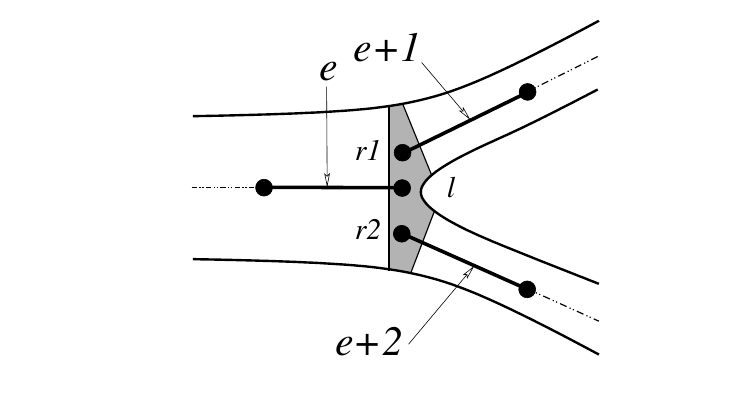
\includegraphics[width=0.5\linewidth]{arterial_tree_bifurcation.png}
    \caption{Arterial tree bifurcation: Notations.}
    \label{fig:arterial-tree}
\end{figure}

For each element $e$, $e+1$ and $e+2$ a function $f$ is continuous but it may be discontinuous at point $x= x_e^u = x^l_{e+1} = x^{l}_{e+2}$ at the interface between three elements (see figure \ref{fig:arterial-tree}). \\
At the bifurcation we have three unknowns $(A_1, U_1)$ in the parent vessel, $(A_{11}, U_{11})$ in the upper vessel and $(A_{12}, U_{12})$ in the lower daughter vessel. \\
The first three equations required to solve the problem are obtained by imposing that the characteristic variables at point $x$ in each vessel should remain constant. Their values are : 
\begin{align}
    W_1 = U_1 + 4 c_1 &= U_1 + 4 \sqrt{\frac{\mu m}{\rho} \left(\frac{A_1}{A_{1_0}} \right)^m} = \text{ constant }. \label{characteristic_1} \\ 
    W_{11} &= U_{11} -  4 \sqrt{\frac{\mu m}{\rho} \left(\frac{A_{11}}{A_{11_0}} \right)^m}= \text{ constant }. \label{characteristic_2} \\ 
    W_{12} &= U_{12} -  4 \sqrt{\frac{\mu m}{\rho} \left(\frac{A_{12}}{A_{12_0}} \right)^m} = \text{ constant }.  \label{characteristic_3}
\end{align}
The other three conditions are required to solve the problem are obtained by the continuity of mass flux and total pressure across the boundary of elements at the bifurcation, i.e. 
\begin{align}
    A_1 U_1 &= U_{11}A_{11} + U_{12}A_{12}. \label{mass_equation}\\
    P_{1_{0}} + \mu \left[ \left( \frac{A_1}{A_{{1}_0}}\right)^m - 1 \right] &= P_{11_{0}} + \mu \left[ \left( \frac{A_{11}}{A_{{11}_0}}\right)^m - 1 \right] . \label{pressure_cont_1} \\
    P_{1_{0}} + \mu \left[ \left( \frac{A_1}{A_{{1}_0}}\right)^m - 1 \right] &= P_{12_{0}} + \mu \left[ \left( \frac{A_{12}}{A_{{12}_0}}\right)^m - 1 \right] . \label{pressure_cont_2}
\end{align}

The six equations given by \ref{characteristic_1}--\ref{pressure_cont_2} define a nonlinear system of algebraic equations that determines the values of $(A_1,U_1)$ in the parent vessel and $(A_{11},U_{11})$, $(A_{12},U_{12})$ in the two daughter vessels at the bifurcation. In the \texttt{deal.II} framework, junction points are detected by identifying non-manifold faces using the function \texttt{get\_non\_manifold\_faces()}.

For the numerical computation, we collect the unknowns into the vector
\[
X =
\begin{pmatrix}
A_1 \\[2pt]
U_1 \\[2pt]
A_{11} \\[2pt]
U_{11} \\[2pt]
A_{12} \\[2pt]
U_{12}
\end{pmatrix},
\]
and solve the nonlinear system defined by \eqref{characteristic_1}--\eqref{pressure_cont_2}. An initial guess for $X$ is obtained from the solution at the previous time level, corresponding to the traces of the numerical solution at the junction in each vessel. The resulting nonlinear system is solved by a Newton-type iteration, which is embedded consistently within the global implicit time-stepping scheme. This procedure ensures that the junction conditions are enforced implicitly at every time step while preserving stability and consistency of the overall discretization.



\begin{remark}
\begin{itemize}
    \item {Newton update.}
Once the corrections $(\delta A_h^{n+1,(k)},\,\delta U_h^{n+1,(k)})$ are computed,
the iterates are updated as
\[
  A_h^{n+1,(k+1)} = A_h^{n+1,(k)} + \delta A_h^{n+1,(k)}, 
  \qquad
  U_h^{n+1,(k+1)} = U_h^{n+1,(k)} + \delta U_h^{n+1,(k)}.
\]
The process is repeated until 
$\|\delta\mathbf{W}_h^{n+1,(k)}\|$ falls below a prescribed tolerance.
\item The increment $\delta\mathbf{W}_h^{n+1,(k)}$ represents the Newton correction at
time level $t_{n+1}$ and iteration $k$, while the Jacobian
$\mathcal{J}^{(k)}$ is obtained by differentiating the discrete residual
$\mathcal{R}^{n+1}(\mathbf{W})$ with respect to $\mathbf{W}$.
The term $\mathbf{H}^{(k)}\delta\mathbf{W}_h^{n+1,(k)}$ originates from the
first-order Taylor expansion of the nonlinear flux
$\mathbf{F}(\mathbf{W})$ about $\mathbf{W}_h^{n+1,(k)}$.
\end{itemize}
\end{remark}
\end{document}